\documentclass[prb,reprint,longbibliography,superscriptaddress,amsmath,amssymb]{revtex4-2}
\usepackage{graphicx}
\usepackage{bm}
\usepackage[dvipsnames]{xcolor}
\usepackage[colorlinks=true,linkcolor=blue,citecolor=blue,urlcolor=blue]{hyperref}

% ---------- symbols (change here only)
\newcommand{\Ts}{T^{*}}
\newcommand{\Tr}{T_{\mathrm{ring}}}
\newcommand{\xiH}{\xi_{\mathrm{H}}}
\newcommand{\Sv}{\mathbf{S}}
\newcommand{\kv}{\mathbf{k}}

% ---------- items the authors must settle; the count is printed in the log
\newcounter{humanbox}
\newcommand{\human}[1]{\stepcounter{humanbox}%
  \par\noindent\fcolorbox{red}{yellow!35}{\parbox{\dimexpr\linewidth-2\fboxsep-2\fboxrule}{\footnotesize\textbf{[AUTHOR]} #1}}\par}
\AtEndDocument{\typeout{=== HUMAN BOXES REMAINING: \thehumanbox\space ===}}

\begin{document}

\title{Ring onset of helical correlations and short-range alignment occur at different temperatures in two-dimensional chiral magnets}

\author{\textcolor{red}{[Authors]}}
\affiliation{Department of Physics, Kyung Hee University, Seoul, Republic of Korea}

\date{\today}

\begin{abstract}
Two-dimensional Heisenberg magnets with Dzyaloshinskii--Moriya interaction (DMI) have no finite-temperature transition, yet simulations and machine-learned order parameters single out a temperature near which helical structure appears. We show that this temperature splits into two crossovers of different origin. The specific-heat maximum $\Ts$ marks short-range alignment on the lattice scale; it exists without DMI and moves by less than 8\% up to $D=0.5J$. The ring-onset temperature $\Tr$, where the maximum of the structure factor leaves $k=0$, is set by the isotropic correlation length reaching a fixed fraction $\alpha\approx0.14$ of the helix pitch, a value the exact large-$N$ solution gives without adjustable parameters. Because the pitch grows as $J/D$ while $\Ts$ is fixed on the lattice scale, the two crossovers meet at $D\approx0.1J$ and their order inverts below, as we confirm at $D=0.05J$. Anisotropy and magnetic fields shift the ring onset of each spin component to where the susceptibility of its DMI partner component equals $J/4D^2$, a criterion that magnetization data can test. The same structure holds on the triangular lattice. An order parameter extracted by a variational autoencoder follows neither crossover; it measures the fraction of spin variance retained by its latent space.
\end{abstract}

\maketitle
\human{Authors, affiliations, and corresponding-author e-mail (title block above is a placeholder).}

%=====================================================================
\section{Introduction}
\label{sec:intro}

In noncentrosymmetric magnets the DMI twists the ferromagnetic state into helices and skyrmion textures whose period $\lambda$ is set by the ratio of exchange $J$ to DMI strength $D$. Above the ordering temperature of bulk helimagnets such as MnSi, the paramagnet already carries chiral fluctuations: neutron scattering finds intensity spread over a sphere of radius $2\pi/\lambda$~\cite{Grigoriev2005,Pappas2017}, and the specific heat shows a broad shoulder next to a sharp first-order peak~\cite{Janoschek2013}. Two accounts of this precursor regime coexist. In the Brazovskii picture the fluctuations on the sphere renormalize the correlation length and drive the transition first order~\cite{TODO-Brazovskii1975,Janoschek2013}. Monte Carlo studies instead attribute the shoulder to a ferromagnetic transition smeared by helical fluctuations~\cite{BelemukStishov2017}.

In three dimensions these questions are compressed into 1--2\,K above a first-order transition. Grigoriev \textit{et al.}~\cite{Grigoriev2011} identified two crossovers there, at inverse correlation lengths $\kappa\approx2k$ and $\kappa\approx k$ of the helical fluctuations, but the thresholds were chosen from inflection points and both lie close to $T_c$. A two-dimensional chiral magnet removes the transition altogether: the Mermin--Wagner theorem forbids long-range order~\cite{TODO-MerminWagner1966}, and every temperature scale is a crossover. This makes the two-dimensional (2D) model a clean setting to ask which feature of the paramagnet sets which temperature, and to follow each feature down to vanishing DMI.

The question has also become practical. A variational autoencoder (VAE) trained on Monte Carlo configurations of the 2D Heisenberg--DMI model produced an order parameter with a characteristic temperature $T\approx0.71J$ that did not depend on $D$~\cite{Yoon2024}. Whether this temperature marks helical order, short-range alignment, or a property of the network is not settled, because the paramagnet has not been resolved into its separate crossovers.

Here we show that two crossovers with different origins exist and that their order depends on $D$. The specific-heat maximum $\Ts$ is a lattice-scale property inherited from the 2D Heisenberg model and nearly independent of $D$. The ring-onset temperature $\Tr$, defined without thresholds by the curvature of the structure factor at $k=0$, is fixed by the isotropic correlation length reaching a constant fraction of $\lambda$. Scale invariance of the 2D continuum model forces $\Tr$ to fall logarithmically as $D\to0$ while $\Ts$ stays put, so the two must cross; Monte Carlo locates the crossing at $D\approx0.1J$ and confirms the inverted order at $D=0.05J$. The ring-onset condition extends to a component-resolved rule under anisotropy and fields, it carries over unchanged to the triangular lattice, and it explains what the VAE order parameter does and does not measure.

Section~\ref{sec:model} defines the model, its exact symmetries, and the two temperatures. Section~\ref{sec:cross} gives their $D$ dependence, Sec.~\ref{sec:theory} the analytic theory of the ring onset, Sec.~\ref{sec:comp} its extension to anisotropy and fields, and Sec.~\ref{sec:lattice} the lattice-independence test. Section~\ref{sec:vae} interprets the VAE order parameter, and Sec.~\ref{sec:disc} discusses the relation to bulk helimagnets and thin films.

%=====================================================================
\section{Model, symmetries, and the two temperatures}
\label{sec:model}

We study classical unit spins on the square lattice (spacing $a=1$) with ferromagnetic exchange and bulk-type (Bloch) DMI,
\begin{equation}
\mathcal H=-J\sum_{\langle ij\rangle}\Sv_i\cdot\Sv_j-D\sum_{\langle ij\rangle}\hat{\mathbf r}_{ij}\cdot(\Sv_i\times\Sv_j),
\label{eq:H}
\end{equation}
where the sums run over nearest-neighbor bonds and $\hat{\mathbf r}_{ij}$ is the bond unit vector. We set $J=1$ and $k_B=1$. Section~\ref{sec:comp} adds a uniaxial anisotropy $-K\sum_i(S_i^z)^2$ and a field $-\mathbf h\cdot\sum_i\Sv_i$. Three exact properties organize all results.

\textit{Gauge structure.} On each bond the two terms combine into $-\tilde J\,\Sv_i\cdot R_{ij}\Sv_j$, with $\tilde J=(J^2+D^2)^{1/2}$ and $R_{ij}$ a rotation about $\hat{\mathbf r}_{ij}$ by $\theta=\arctan(D/J)$. The DMI is therefore a constant SO(3) gauge field: it fixes the twist per bond, and hence the helix wave number $q=\theta$ along a bond, independently of temperature. The pitch is $\lambda=2\pi/\arctan(D/J)$.

\textit{Scale invariance.} In the continuum limit the energy is
\begin{equation}
E=\int d^2r\,\Big[\frac{J}{2}(\nabla\Sv)^2+D\,\Sv\cdot(\nabla\times\Sv)\Big].
\label{eq:cont}
\end{equation}
Under $\mathbf r\to\ell\mathbf r$ the exchange term is invariant in two dimensions while the DMI term scales by $\ell$. Choosing $\ell=J/D$ removes $D$ entirely, so at fixed $T/J$ the continuum model depends on $D$ only through the ratio of the lattice cutoff to the pitch. Any dimensionless observable is thus a function $F(T/J,\lambda/a)$. This has two consequences. A quantity fixed on the lattice scale, such as the energy and its temperature derivative, approaches its $D=0$ form as $\lambda/a\to\infty$. A quantity fixed on the scale $\lambda$ must be decided by comparing a lattice-scale length with $\lambda$.

\textit{Parity.} Spatial inversion maps $D\to-D$, so every thermodynamic quantity is even in $D$.

\textit{Lattice anisotropy.} The square lattice breaks the continuous rotation of the helix direction. Expanding the lattice dispersion gives $E(\phi)\approx E_0+(D^4/32J^3)\cos4\phi$ for a helix at angle $\phi$ to a bond, with diagonal helices lowest. The amplitude is below $2\times10^{-3}J$ for $D\le0.5J$ and does not affect the paramagnetic crossovers studied here (Sec.~\ref{sec:lattice} tests this directly).

\textit{Definitions.} The specific-heat temperature $\Ts$ is the maximum of $C=dU/dT$, with $U$ the energy per spin. The ring-onset temperature $\Tr$ is defined from the total structure factor $S(\kv)=N^{-1}\sum_a\langle|S_a(\kv)|^2\rangle$. Writing
\begin{equation}
S(\kv)^{-1}=r+c_1\hat k^2+c_2\hat k^4+\dots,
\label{eq:fit}
\end{equation}
with the lattice momentum $\hat k^2=4\sin^2(k_x/2)+4\sin^2(k_y/2)$.
$\Tr$ is where $c_1$ changes sign. Above $\Tr$ the maximum of $S(\kv)$ sits at $k=0$; below it the maximum moves to a ring near $|\kv|=q$ (Fig.~\ref{fig:ring}). The definition contains no threshold, and $\Tr$ is a crossover without thermodynamic singularity. In the competing-interaction literature this locus is called a Lifshitz line; we avoid that name because it suggests a multicritical Lifshitz point and because the line depends on how the spin components are combined (Sec.~\ref{sec:theory}).

\begin{figure}[tb]
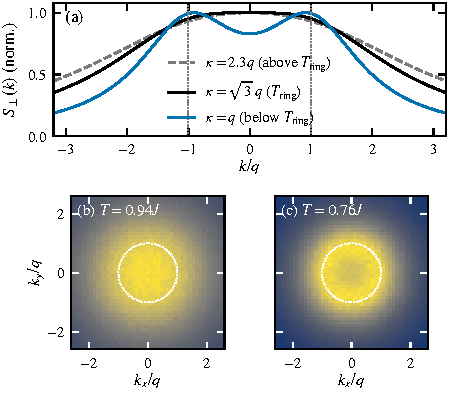
\includegraphics[width=\columnwidth]{figures/fig1_ring_onset.pdf}
\caption{The ring onset is the temperature at which the two helical branches of the structure factor become resolved. (a) Gaussian transverse structure factor, Eq.~\eqref{eq:lor}, for three widths $\kappa$: the branches at $\pm q$ merge into one maximum at $k=0$ for $\kappa>\sqrt3\,q$ and separate below. (b), (c) Total $S(\kv)$ from Monte Carlo at $D=0.3J$ ($L=176$, four seeds) above and below $\Tr=0.854J$, each normalized to its maximum. The dotted circle marks $|\kv|=q$.}
\label{fig:ring}
\end{figure}

The scale argument already predicts the outcome. The 2D Heisenberg correlation length grows as $\xiH\propto\exp(2\pi J/T)$ at low temperature~\cite{TODO-Polyakov1975,TODO-HasenfratzNiedermayer1991}, so a condition $\xiH(\Tr)=\alpha\lambda$ with constant $\alpha$ gives
\begin{equation}
\frac{1}{\Tr}\simeq\frac{1}{2\pi J}\ln\frac{\alpha\lambda}{a}+\dots\ \xrightarrow{\;D\to0\;}\ \infty .
\label{eq:log}
\end{equation}
$\Tr$ therefore vanishes logarithmically as $D\to0$, while $\Ts$ stays at its $D=0$ value. The two crossovers must cross at some $D$.

%=====================================================================
\section{Two crossovers and their order}
\label{sec:cross}

The specific-heat maximum exists without DMI and hardly moves with $D$, while the ring onset rises steeply with $D$; the two cross near $D=0.1J$ (Fig.~\ref{fig:temps}, Table~\ref{tab:temps}).

\begin{figure}[tb]
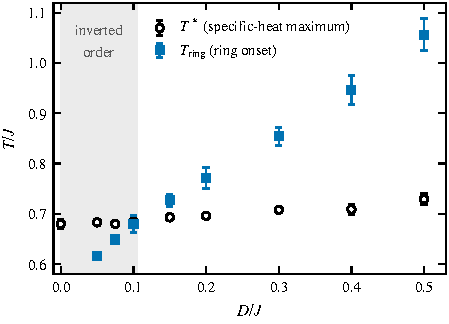
\includegraphics[width=\columnwidth]{figures/fig2_two_temperatures.pdf}
\caption{The specific-heat maximum $\Ts$ (open circles) and the ring-onset temperature $\Tr$ (squares) cross near $D=0.1J$, and $\Tr<\Ts$ below. Monte Carlo on the square lattice with $L/\lambda\ge4$; error bars combine the statistical error and the dependence on the fitting window (Appendix~\ref{app:mc}). The shaded region marks the inverted order.}
\label{fig:temps}
\end{figure}

\textit{Specific-heat maximum.} At $D=0$ the specific heat has a broad maximum at $\Ts=0.680(9)J$, as expected for the 2D Heisenberg model, whose correlation length there is $\xiH\approx9.5a$. Turning on $D$ shifts $\Ts$ by $+0.4\%$ at $D=0.1J$ and $+7\%$ at $D=0.5J$. The maximum is thus a lattice-scale feature, set where short-range alignment builds up over about ten lattice spacings, in line with the scale argument of Sec.~\ref{sec:model}. The precise functional form of the small shift is not resolved by our data: a form linear in $|D|$ fits as well as a crossover from $D^2$ to $|D|$ at $D\approx a/\xiH(\Ts)$ (Appendix~\ref{app:mc}).

\textit{Ring onset.} $\Tr$ increases from $0.68J$ at $D=0.1J$ to $1.06J$ at $D=0.5J$. Above $\Ts$ the correlations are short ranged ($\xiH<10a$), yet the structure factor already has its maximum on the ring whenever $T<\Tr$. For $D>0.1J$ helical correlations therefore become visible before short-range alignment sets in.

\textit{Inversion.} Below $D\approx0.1J$ the order reverses. At $D=0.05J$ we find $\Tr-\Ts=-0.067(7)J$ for $L=512$ and $-0.063(8)J$ for $L=1024$ ($L/\lambda=4$ and 8). At $D=0.075J$ the difference is $-0.032(8)J$. Linear interpolation places the crossing at $D\approx0.105J$. In the inverted regime short-range alignment comes first, and the ring appears only at lower temperature, when $\xiH$ has grown to a fraction of the now longer pitch.

\begin{table}[tb]
\caption{Crossover temperatures from Monte Carlo on the square lattice (units of $J$). Errors in parentheses combine statistics and fitting window. $\Tr^{\rm ext}$ is obtained from fits extrapolated to vanishing window (Appendix~\ref{app:mc}); at $D=0.05J$ it is the mean of $L=512$ (0.629) and 1024 (0.627). $L$ refers to the $\Tr$ runs.}
\label{tab:temps}
\begin{ruledtabular}
\begin{tabular}{@{}cccccc@{}}
$D$ ($J$) & $\lambda$ ($a$) & $L$ & $\Ts$ & $\Tr$ & $\Tr^{\rm ext}$ \\
\hline
0     & --    & 512       & 0.680(9)  & --        & --          \\
0.05  & 125.8 & 512/1024 & 0.683(5)  & 0.616(5)  & 0.628 \\
0.075 & 83.9  & 384       & 0.680(2)  & 0.649(8)  & 0.659 \\
0.1   & 63.0  & 512       & 0.684(5)  & 0.679(17) & 0.682 \\
0.15  & 42.2  & 336       & 0.693(3)  & 0.727(12) & 0.740 \\
0.2   & 31.8  & 256       & 0.696(2)  & 0.771(21) & 0.775 \\
0.3   & 21.6  & 176       & 0.708(5)  & 0.854(18) & 0.860 \\
0.4   & 16.5  & 128       & 0.709(10) & 0.946(29) & 0.969 \\
0.5   & 13.5  & 112       & 0.729(11) & 1.056(32) & 1.065 \\
\end{tabular}
\end{ruledtabular}
\human{Confirm the system sizes and combination (cooling/heating, $L/\lambda=4$ and 8) behind the $\Ts$ column; the $\Ts$ values may come from runs at sizes different from the listed $L$.}
\end{table}

%=====================================================================
\section{Theory of the ring onset}
\label{sec:theory}

The ring appears when the width of each helical branch drops below $\sqrt3$ times its distance from the origin, and this happens at a fixed ratio $\alpha=\xiH(\Tr)/\lambda\approx0.14$ that the large-$N$ solution reproduces without parameters (Fig.~\ref{fig:alpha}).

\textit{Resolution of two branches.} Consider fluctuations with wave vector along $x$. The DMI couples $S_y$ and $S_z$, while $S_x$ (parallel to $\kv$) is not coupled. With a common Gaussian mass $A$ and stiffness $J$, the transverse response splits into chiral branches $Jk^2-2Dk+A$ and $Jk^2+2Dk+A$. Each transverse component sees both branches,
\begin{equation}
S_{zz}(k)\propto\frac{1}{(k-q)^2+\kappa^2}+\frac{1}{(k+q)^2+\kappa^2},
\label{eq:lor}
\end{equation}
with $q=D/J$ and $\kappa^2=A/J-q^2$, where $\kappa$ is the inverse correlation length of the helical fluctuations. The curvature at $k=0$ is proportional to $6q^2-2\kappa^2$. The ring therefore appears in a transverse component when $\kappa=\sqrt3\,q$, which is the condition for two equal Lorentzians to be resolved (vanishing second derivative midway between them). The longitudinal component is a single Lorentzian at $k=0$ and delays the onset in the total $S(\kv)$, which turns over at $\kappa=(5/3)^{1/2}q$, equivalently $A=8D^2/3J$. Neither condition contains a threshold. They make precise the crossover $\kappa\approx2k$ identified from inflection points in bulk helimagnets~\cite{Grigoriev2011}.

\textit{Gaussian estimate.} In terms of the isotropic correlation length $\xi=(J/A)^{1/2}$, the total-$S(\kv)$ condition reads $q\xi=(3/8)^{1/2}$, or $\xi/\lambda=0.098$. With the high-temperature mass $A=3T-4J$ this gives $\Tr=4J/3+8D^2/9J$. The scale $\xi\propto\lambda$ is right, but the temperature is not, because the Gaussian theory misses the exponential growth of $\xiH$.

\textit{Exact large-$N$ solution.} The spherical (large-$N$) version of Eq.~\eqref{eq:H} is solvable on the lattice. Its eigenvalues are $\lambda_\pm(\kv)=J_0(\kv)\pm2D|s(\kv)|$ and $\lambda_0(\kv)=J_0(\kv)$, with $J_0=2J(\cos k_x+\cos k_y)$ and $|s|=(\sin^2k_x+\sin^2k_y)^{1/2}$. The Lagrange multiplier $\mu$ follows from
\begin{equation}
1=\frac{T}{N}\sum_{\kv}\sum_{a=\pm,0}\frac{1}{\mu-\lambda_a(\kv)},
\label{eq:largeN}
\end{equation}
and the ring onset of the total $S(\kv)$ is exactly $\mu-4J=8D^2/3J$. Evaluating $\xiH$ from the same solution at $D=0$ gives $\alpha=0.137$ for $D\to0$, decreasing slowly to $0.111$ at $D=0.5J$ (Fig.~\ref{fig:alpha}). The large-$N$ temperatures themselves differ from the Heisenberg values, but the ratio $\alpha$ is the quantity the scale argument requires, and it is nearly constant.

The large-$N$ solution has no specific-heat maximum: $C$ rises monotonically to its low-temperature value. The maximum at $\Ts$ is therefore a property of fixed-length spins beyond leading order in $1/N$. The two crossovers have different theoretical status: $\Tr$ is captured by a free theory with the correct correlation length, $\Ts$ is not.

\begin{figure}[tb]
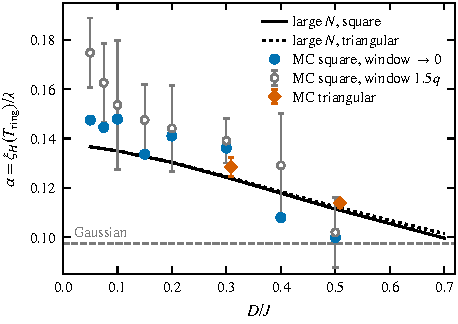
\includegraphics[width=\columnwidth]{figures/fig3_alpha.pdf}
\caption{The Heisenberg correlation length at the ring onset is a fixed fraction of the pitch. Filled circles: Monte Carlo on the square lattice with the fitting window extrapolated to zero; open circles: fixed window $1.5q$, with errors combining statistics and window dependence. Diamonds: triangular lattice ($L=96$, mean over windows $1.0q$--$1.5q$, shifted by $+0.008$ in $D$ for visibility). Solid and dotted lines: exact large-$N$ solutions on the square and triangular lattices. Dashed line: Gaussian value 0.098. $\xiH(T)$ is taken from $D=0$ simulations on the same lattice.}
\label{fig:alpha}
\end{figure}

\textit{Monte Carlo.} Combining the measured $\Tr$ with $\xiH(T)$ at $D=0$, Monte Carlo gives $\alpha$ between 0.134 and 0.148 for $D\le0.3J$ when the fitting window is extrapolated to zero. Both the value and the slow decrease at larger $D$ agree with the large-$N$ result. The fixed-window estimator gives larger $\alpha$ at small $D$, up to 0.175 at $D=0.05J$. The difference is a known bias of truncated fits and is amplified by the exponential temperature dependence of $\xiH$: a shift of $0.01J$ in $\Tr$ changes $\alpha$ by about 15\%. We therefore quote $\alpha\approx0.14$ with a systematic uncertainty of about 10\%. The decrease of $\alpha$ at $D\ge0.4J$ appears in both theory and simulation; there $\Tr$ lies where $\xiH$ is only one or two lattice spacings and lattice corrections to the continuum enter.

%=====================================================================
\section{Anisotropy and fields: a component-resolved rule}
\label{sec:comp}

With anisotropy or a field the spin components no longer share one mass, and the ring onset splits by component. Each component develops its ring when the uniform susceptibility of its DMI partner reaches $J/4D^2$; Monte Carlo confirms this threshold to within about 10\% on average (Table~\ref{tab:comp}).

\textit{Rule.} For wave vector along $x$ the DMI couples $S_z$ to the in-plane transverse component $S_y$. Eliminating $S_y$ at Gaussian level gives
\begin{equation}
S_{zz}(k)^{-1}=A_z+Jk^2-\frac{4D^2k^2}{A_y+Jk^2}\ \Rightarrow\ c_1^{(zz)}=J-\frac{4D^2}{A_y},
\label{eq:rule}
\end{equation}
so the ring of $S_{zz}$ appears when $\chi_y=1/A_y$ reaches $J/4D^2$, and symmetrically for $S_{yy}$ with $\chi_z$. Without anisotropy all masses are equal and the rule reduces to $\kappa=\sqrt3\,q$ of Sec.~\ref{sec:theory}. The rule says which susceptibility to watch: the onset of one component is controlled by the response of the other.

\textit{Uniaxial anisotropy.} An easy axis ($K>0$) raises $\chi_z$, so the in-plane transverse ring appears first; an easy plane ($K<0$) reverses the order. For unit spins the high-temperature expansion $\langle(S^z)^2\rangle=1/3+(4/45)K/T$ shifts the $z$ mass by $(4/5)K$, not by the $2K$ of the spherical model. The splitting is therefore small for $|K|\ll D^2/J$.

\textit{Field normal to the plane.} For a field along $z$ the transverse susceptibility of a rotation-invariant system equals $m/h$ exactly. The ring of $S_{zz}$ therefore appears where the magnetization curve satisfies
\begin{equation}
\frac{m(\Tr,h)}{h}=\frac{J}{4D^2},
\label{eq:mh}
\end{equation}
a condition fixed by magnetization data alone. In the large-$N$ solution $\Tr(h)=\Tr(0)[1-(h/h_L)^2]$ with $h_L=4D^2/J$, the same scale as the field range of the skyrmion lattice.

\textit{Field in the plane.} For $\mathbf h$ along $x$, both partners of a helix with $\kv\parallel\mathbf h$ are transverse to the field and share $\chi_\perp=m/h$, whereas a helix with $\kv\perp\mathbf h$ has the longitudinal component as partner. The ring therefore appears first along the field direction and becomes anisotropic.

\begin{table*}[tb]
\caption{Monte Carlo test of the component rule at $D=0.3J$ ($L=96$, four seeds, units of $J$). The Gaussian threshold for the partner susceptibility is $J/4D^2=2.78$.}
\label{tab:comp}
\begin{ruledtabular}
\begin{tabular}{llllll}
Perturbation & $\Tr$ of $S_{zz}$ & $\Tr$ of in-plane transverse & Partner susceptibility on $S_{zz}$ onset & Shift of $\Ts$ \\
\hline
none                  & 0.916(13) & 0.924(9)  & 3.38(19)    & -- ($\Ts=0.701(2)$) \\
$K=+0.05$ (easy axis) & 0.945(15) & 0.951(17) & 2.87(17)    & $-0.2(4)\%$ \\
$K=-0.05$ (easy plane)& 0.964(16) & 0.877(23) & 2.93(13)    & $+0.2(3)\%$ \\
$h_z=0.05$            & 0.907(16) & 0.891(17) & $m/h=3.04$  & $+0.8(5)\%$ \\
$h_z=0.10$            & 0.888(69) & 0.712(56) & $m/h=2.97$  & $+5.8(4)\%$ \\
$h_x=0.10$            & $\kv\parallel\mathbf h$: 0.851(55) & $\kv\perp\mathbf h$: 0.714(20) & $m/h=3.55$ & $+10.0(4)\%$ \\
\end{tabular}
\end{ruledtabular}
\end{table*}

\textit{What the simulation confirms.} On every onset line the partner susceptibility lies between 2.9 and 3.6, 1.03--1.28 times the Gaussian value, without fitting. The easy-plane splitting has the predicted sign and size, $0.087(28)J$. The easy-axis splitting predicted for $K=+0.05J$ is below our resolution. In an in-plane field the ring weight concentrates along the field: $\langle\cos2\phi\rangle$ of the ring grows from 0.02 at $T=0.9J$ to 0.14 at $T=0.6J$, compared with $|\langle\cos2\phi\rangle|<0.01$ without field, and the onset for $\kv\parallel\mathbf h$ lies above that for $\kv\perp\mathbf h$.

\textit{Response of $\Ts$.} Anisotropy of $\pm0.05J$ leaves $\Ts$ unchanged within 0.4\%, while a field of $0.1J$ raises it by 6\% (normal) and 10\% (in plane). The specific-heat maximum thus responds to fields on the scale $0.1J$ but not to weak anisotropy. We have no quantitative theory for this response; the factor 1.7 between in-plane and normal fields is an observation.

%=====================================================================
\section{Lattice independence}
\label{sec:lattice}

On the triangular lattice both temperatures are rescaled by a single factor of 1.61, and the dimensionless relations $\alpha$ and $\Tr/\Ts$ agree with the square lattice within errors (Table~\ref{tab:tri}).

\textit{How to compare lattices.} For a lattice with coordination $z$ and unit-cell area $A_c$, the gradient expansion of Eq.~\eqref{eq:H} gives stiffnesses per unit area
\begin{equation}
\rho_J=\frac{zJ}{4A_c},\qquad \rho_D=\frac{zD}{4A_c},\qquad q=\frac{\rho_D}{\rho_J}=\frac{D}{J}.
\label{eq:rho}
\end{equation}
The same $J$ and $D$ therefore give the same pitch on both lattices ($\lambda=21.6a$ and $21.4a$ at $D=0.3J$ from the exact dispersions). Temperatures should be compared in units of $\rho_J$, which is $J$ on the square and $\sqrt3\,J$ on the triangular lattice. Even then the absolute temperatures differ by a lattice-dependent constant, because $\xiH$ depends exponentially on $T/\rho_J$ with a nonuniversal prefactor. What the scale argument predicts to be lattice independent is the relation expressed through $\xiH$, namely $\alpha$.

\textit{Large $N$.} The ring-onset condition on any Bravais lattice is $\mu-zJ=(2/3)zD^2/J$. Solving both lattices with the same code gives $\alpha$ equal within 1\% for $D\le0.5J$, including its decrease with $D$ (Fig.~\ref{fig:alpha}). The ratio of $\Tr/\rho_J$ between the lattices is 0.96 at $D=0.05J$ and 0.92 at $D=0.5J$: lattice effects in the temperature shrink with decreasing $D$, but only logarithmically. The test is therefore most stringent at intermediate and large $D$, which is where we performed it.

\begin{table}[tb]
\caption{Square versus triangular lattice (Monte Carlo, units of $J$). Triangular lattice: $L=96$, three seeds; ranges reflect fitting windows $1.0q$--$1.5q$.}
\label{tab:tri}
\begin{ruledtabular}
\begin{tabular}{llll}
Quantity & Square & Triangular & Ratio \\
\hline
$\Ts$, $D=0$ & 0.680(9) & 1.100(1) & 1.62 \\
$\xiH(\Ts)$, $D=0$ & $9.5a$ & $9.65a$ & 1.02 \\
$\Tr$, $D=0.3J$ & 0.852--0.856 & 1.377--1.400 & 1.61--1.64 \\
$\Tr$, $D=0.5J$ & 1.049--1.069 & 1.688--1.707 & 1.60--1.61 \\
$\alpha$, $D=0.3J$ & 0.133--0.136 & 0.124--0.131 & \\
$\alpha$, $D=0.5J$ & 0.114--0.120 & 0.112--0.115 & \\
$\Tr/\Ts$, $D=0.3J$ & 1.20--1.21 & 1.21--1.23 & \\
$\Tr/\Ts$, $D=0.5J$ & 1.44--1.47 & 1.45--1.47 & \\
Shift of $\Ts$, $D=0.3J$ & $+4.1\%$ & $+3.1(2)\%$ & \\
Shift of $\Ts$, $D=0.5J$ & $+7.2\%$ & $+5.7(3)\%$ & \\
\end{tabular}
\end{ruledtabular}
\end{table}

\textit{Result.} A single factor of 1.61 converts both temperatures, 7\% below $\sqrt3$ and equal to the large-$N$ value $0.93\sqrt3$. The specific-heat maximum occurs at the same correlation length, $\xiH\approx9.6a$, on both lattices. Since the crossing is fixed by $\xiH(\Ts)=\alpha\lambda$, the triangular lattice should show the same crossing near $D\approx2\pi\alpha a/\xiH(\Ts)\approx0.09J$; we have not simulated that regime. The shift of $\Ts$ with $D$ is somewhat smaller on the triangular lattice, a difference of about one standard deviation given the square-lattice errors.

%=====================================================================
\section{What a VAE order parameter measures}
\label{sec:vae}

The order parameter that a VAE extracts from these configurations follows neither $\Ts$ nor $\Tr$. In the linear limit it is the fraction of spin variance that the latent space retains, and its characteristic temperature is set by the latent dimension.

\textit{Linear theory.} Reference~\cite{Yoon2024} trained a VAE on configurations pooled over temperatures and defined $\eta=\langle|\tilde\Sv|\rangle$ from the decoder output $\tilde\Sv$. For a linear encoder and decoder with Gaussian likelihood, the optimum is probabilistic principal component analysis~\cite{TODO-TippingBishop1999}: the latent space keeps the $n_z$ covariance modes of the pooled data whose variance $\bar s$ exceeds the decoder noise $\theta$, each with gain $g=1-\theta/\bar s$. For translation-invariant data these modes are Fourier modes, and
\begin{equation}
\eta^2(T)\simeq\frac{1}{N}\sum_{\kv\in\text{kept}}g_{\kv}^2\,S(\kv,T).
\label{eq:eta}
\end{equation}
The kept modes are those with the largest variance in the pooled data: small $k$ at $D=0$ and the ring at finite $D$. The value of $\eta$ at temperature $T$ is therefore the share of that temperature's spin variance carried by those modes.

\textit{Consequences.} Three predictions follow and none involves chirality. (i) $\eta(T)$ has the same shape at $D=0$ as at finite $D$, since only the location of the kept modes changes. (ii) The characteristic temperature of $\eta$ depends on $n_z$: at $D=0.3J$ the temperature where $\eta$ reaches half its low-temperature value is $0.46J$, $0.58J$, and $0.71J$ for $n_z=25$, 100, and 400. (iii) At fixed $n_z=100$ it moves down with $D$, from $0.62J$ at $D=0$ to $0.49J$ at $D=0.5J$, unlike either crossover.

\textit{Comparison with a trained VAE.} At $D=0.3J$ the linear prediction agrees with a nonlinear VAE trained on a quarter of the data for 30 epochs, with mean deviation 0.010 in $\eta$ on held-out configurations for $T=0.2J$--$0.7J$ (Fig.~\ref{fig:vae}). The linear theory gives a smooth decrease of $\eta$ and does not reproduce the sharp drop near $0.71J$ reported in Ref.~\cite{Yoon2024}. Identifying the origin of that sharpness requires full nonlinear training at $D=0$, which we leave open.

\begin{figure}[tb]
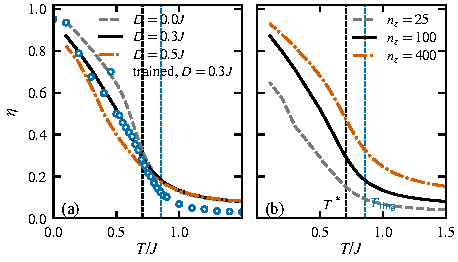
\includegraphics[width=\columnwidth]{figures/fig4_vae.pdf}
\caption{A VAE order parameter tracks the retained spin variance, not a crossover. (a) Linear theory, Eq.~\eqref{eq:eta}, for $D=0$, $0.3J$, and $0.5J$ at $n_z=100$ (lines), and a nonlinear VAE at $D=0.3J$ evaluated on held-out configurations (circles; trained on a quarter of the data for 30 epochs). (b) Linear theory at $D=0.3J$ for $n_z=25$, 100, and 400. Dashed vertical lines: $\Ts$ and $\Tr$ at $D=0.3J$. All curves for $L=128$.}
\label{fig:vae}
\end{figure}

This refines the interpretation of Ref.~\cite{Yoon2024}. The temperature near $0.7J$ at which its order parameter changes most is close to $\Ts$ and nearly independent of $D$, but the linear theory shows that a similar temperature arises from the latent dimension and the variance spectrum alone. A VAE order parameter becomes informative about helical order only when compared with the threshold-free scales $\Ts$ and $\Tr$.

%=====================================================================
\section{Discussion}
\label{sec:disc}

The two crossovers are set on different length scales. Short-range alignment is decided when $\xiH$ reaches about ten lattice spacings, a condition that does not know about $\lambda$. The ring is decided when $\xiH$ reaches about one seventh of $\lambda$, a condition that does not know about the lattice. Scale invariance of the 2D continuum model turns this into a definite statement: one temperature is fixed, the other falls logarithmically with $D$, and their order must invert at small $D$.

\textit{Relation to bulk helimagnets.} In three dimensions the same two scales exist, but both crossovers lie within 1--2\,K of a first-order transition, which makes their $D$ dependence hard to follow~\cite{Grigoriev2011,Janoschek2013}. The broad specific-heat shoulder of MnSi has been read as a consequence of Brazovskii renormalization~\cite{Janoschek2013} and as a ferromagnetic transition smeared by helical fluctuations~\cite{BelemukStishov2017}. In two dimensions the specific-heat maximum exists without DMI, sits at the same correlation length on two lattices, and has a $D$ dependence unlike that of the ring. The 2D results thus separate the alignment feature from the chiral one, which is the distinction the second reading draws.

\textit{Where the model applies.} The scale argument of Sec.~\ref{sec:model} becomes exact as $\lambda/a\to\infty$, and the measured $\alpha$ is constant within errors for $\lambda\ge22a$. Chiral films and interfaces typically have pitches of tens to hundreds of lattice spacings, so they lie in the regime where the continuum description and the inverted order apply. The model predicts that in such systems the specific-heat or susceptibility anomaly appears before helical correlations become resolvable in small-angle scattering or real-space imaging. The component rule gives a test that needs no fitting: in a field normal to the film, the ring of the out-of-plane component appears where $m/h=J/4D^2$, with $J$ and $D$ from spin-wave measurements. Uniaxial anisotropy, which most films have, enters the rule only through the partner susceptibility, as Sec.~\ref{sec:comp} shows.

\textit{Range of validity.} All temperatures are crossovers. Their values depend on the estimator at the level of $0.01J$ for $\Tr$, which translates into a systematic uncertainty of about 10\% in $\alpha$ (Appendix~\ref{app:mc}). The inversion is established on the square lattice at $D=0.05J$ and $0.075J$ with two system sizes; on the triangular lattice it is predicted from the measured $\xiH(\Ts)$ and $\alpha$ but not simulated. The triangular-lattice comparison uses one system size, $L=96$ ($L/\lambda=4.5$--7). The functional form of the small shift of $\Ts$ with $D$ is not determined, and the easy-axis splitting of the ring onset is below our resolution at $K=0.05J$. The VAE analysis rests on the linear theory and one nonlinear pilot; the sharp drop reported for the full VAE is not explained.

%=====================================================================
\section{Conclusion}
\label{sec:concl}

In two-dimensional chiral magnets, the temperature at which helical correlations become visible and the temperature of short-range alignment are distinct crossovers with different origins. The ring onset follows from the resolution of the two helical branches of the structure factor and occurs at $\xiH\approx0.14\lambda$, a ratio that the exact large-$N$ solution reproduces and that is the same on the square and triangular lattices. The specific-heat maximum is inherited from the 2D Heisenberg model and barely depends on $D$. Because $\lambda$ grows as $J/D$, the ring onset falls below the specific-heat maximum for $D<0.1J$, that is, for pitches longer than about 60 lattice spacings. Under anisotropy and fields the ring onset becomes component resolved and is controlled by the partner susceptibility, $J/4D^2$, which magnetization measurements can access. These threshold-free scales also provide the reference against which machine-learned order parameters should be read.

\begin{acknowledgments}
\human{Funding statement and grant number (NRF), and author contributions if required.}
\human{AI-use disclosure: confirm tools, versions, and scope. Draft: ``Simulation and analysis codes and parts of the manuscript text were prepared with the assistance of an AI model; the authors checked all results against independent implementations and analytic limits and take responsibility for the content.''}
\end{acknowledgments}

\section*{Data availability}
\human{Choose the APS data-availability statement. Draft: codes, summary data, and figure scripts are available at github.com/cywon-commits/chiral-magnet-two-temperatures (archive DOI to be created on Zenodo); raw spin configurations (about 32\,GB) are available from the authors upon request.}

%=====================================================================
\appendix

\section{Monte Carlo and estimators}
\label{app:mc}

\textit{Simulations.} We used single-site Metropolis updates combined with energy-conserving over-relaxation, cooling from high temperature. System sizes satisfy $L/\lambda\ge4$ ($L=112$--1024 on the square lattice). Each temperature received 1000 equilibration and 4000--6000 measurement sweeps; integrated autocorrelation times of the energy are below 12 sweeps everywhere. Errors are standard errors over two to four independent seeds, combined with block bootstrap where larger.
\human{Add the details of the $\Ts$ runs (cooling and heating branches, sizes $L/\lambda=4$ and 8, temperature spacing) and check the sweep numbers against the run logs.}

\textit{$\Ts$.} $C=dU/dT$ is computed by central differences on a $0.01J$ grid near the maximum, and the peak is located by a quadratic fit over half-width $0.04J$. Half the spread over half-widths $0.03J$--$0.05J$ is added as a systematic error.

\textit{$\Tr$.} The structure factor is fitted by Eq.~\eqref{eq:fit} inside $|\kv|\le wq$. $\Tr$ is the lowest-temperature sign change of $c_1/r$ for $w=1.5$, and half the spread over $w=1.2$--2.0 is the systematic error. Truncating the expansion biases $\Tr$ downward as $w$ grows. Extrapolating $\Tr$ linearly in $w^2$ to $w\to0$ raises it by $0.005J$--$0.012J$; these values appear in the last column of Table~\ref{tab:temps} and as filled symbols in Fig.~\ref{fig:alpha}.

\textit{$\xiH$ and $\alpha$.} $\xiH(T)$ is obtained from the $D=0$ structure factor at $L=512$ by the same fit, $\xiH=(c_1/r)^{1/2}$, and interpolated logarithmically in $T$.

\textit{Finite size.} At $D=0.05J$, $L=512$ and 1024 ($L/\lambda=4$ and 8) give $\Tr=0.616J$ and $0.617J$ and $\Ts=0.683J$ and $0.681J$.

\textit{Shift of $\Ts$.} The shift $\Delta\Ts/\Ts(0)$ is fitted equally well by $b|D|$ and by $b[(D^2+D_0^2)^{1/2}-D_0]$ with $D_0=a/\xiH(\Ts(0))=0.105J$ and $b\approx0.19$; a pure $D^2$ form is disfavored only when the errors of $dU/dT$ alone are used.

\section{Large-\texorpdfstring{$N$}{N} details}
\label{app:largeN}

The constraint, Eq.~\eqref{eq:largeN}, is solved on a $1024\times1024$ grid of $\kv$ shifted by half a spacing to avoid $\kv=0$. The energy is $U=(3T-\mu)/2$ and $C=dU/dT$. The ring-onset condition follows from the $k^2$ coefficient of $S(\kv)^{-1}$ at $k=0$, which requires $\mu-zJ=(2/3)zD^2/J$ on any Bravais lattice with nearest-neighbor bonds.

\bibliography{refs}

\end{document}
